\label{chap.3}
\section{Study area}
The five districts were chosen because they share three properties that the system depends on.

\begin{enumerate}
	\item \textbf{Recurring drought exposure.} Beed, Latur and Osmanabad lie on the Marathwada plateau; Ahmednagar and Solapur lie in the semi-arid rain-shadow belt of western Maharashtra. All five belong to the State's traditional scarcity zone, with a long record of failed or delayed monsoons.
	\item \textbf{Consistent multi-source data.} Each district has 26 years of daily weather (2000--2025), 23 years of crop statistics (2000--01 to 2022--23) and Census 2011 demographics, which gives a uniform base for modelling.
	\item \textbf{Official contingency plans exist.} An ICAR-format District Agriculture Contingency Plan is available for each of the five, and these plans are the knowledge base the recommendation layer is built on.
\end{enumerate}

Table~\ref{tab:climate} summarises the climate of the five districts as found during exploratory analysis, and Figure~\ref{fig:kharifrain} shows how much the Kharif-season rainfall varies from year to year.

\begin{table}[H]
	\centering
	\caption{Rainfall characteristics of the five districts, 2000--2025 (NASA POWER daily data)}
	\label{tab:climate}
	\small
	\begin{tabular}{lp{3cm}p{2.4cm}p{4cm}}
		\toprule
		\textbf{District} & \textbf{Mean annual rain (mm)} & \textbf{Jun--Sep share} & \textbf{Longest dry spell (days/yr, avg.)} \\
		\midrule
		Ahmednagar & 677 & 80.1\% & 75.7 \\
		Beed       & 721 & 80.5\% & 72.2 \\
		Latur      & 762 & 78.9\% & 70.4 \\
		Osmanabad  & 752 & 76.8\% & 71.0 \\
		Solapur    & 622 & 73.8\% & 76.3 \\
		\bottomrule
	\end{tabular}
\end{table}

\begin{figure}[H]
	\centering
	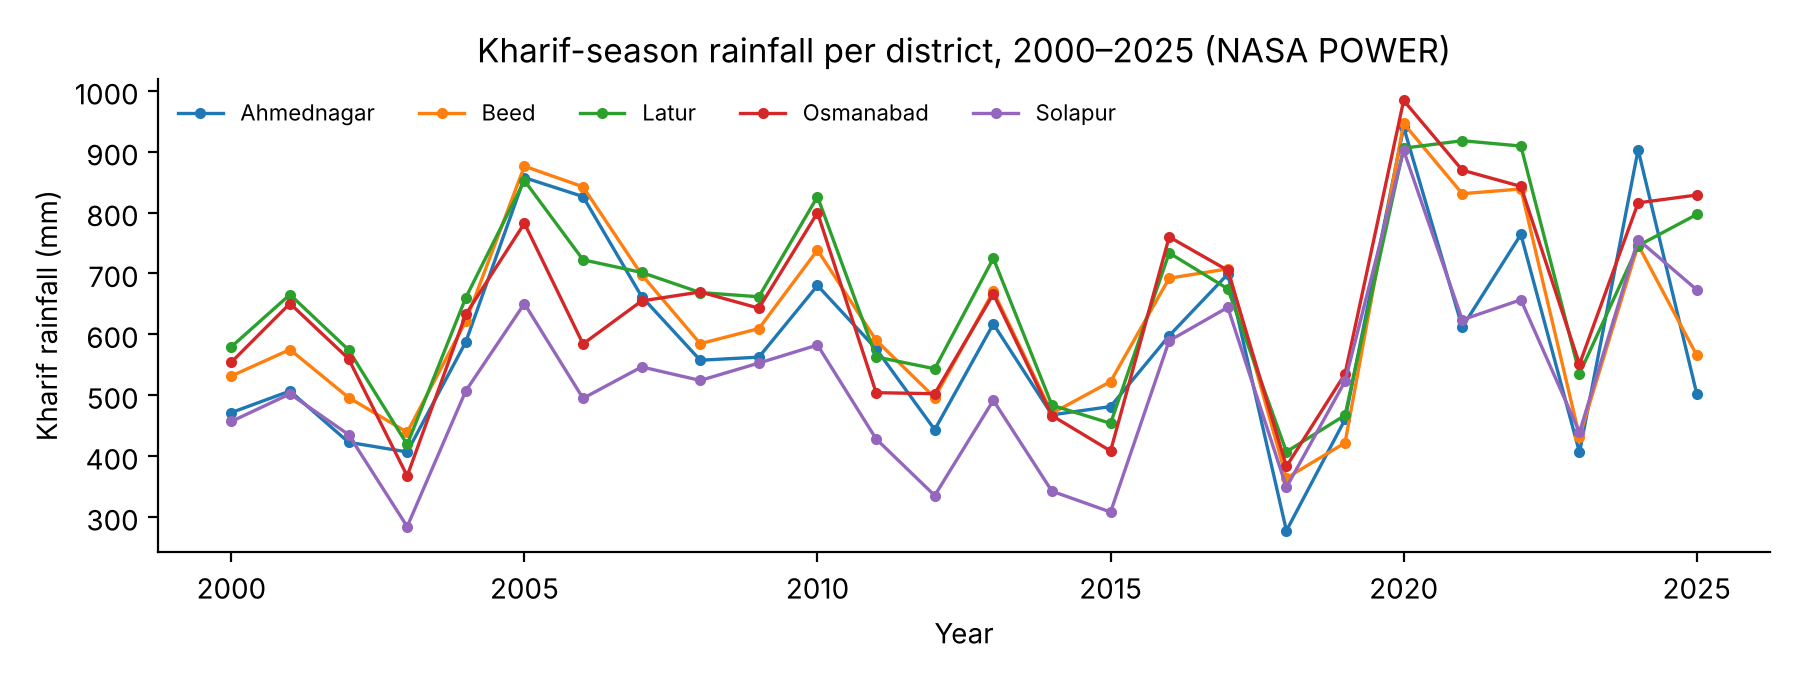
\includegraphics[width=\textwidth]{kharif_rain.png}
	\caption{Kharif-season rainfall in each district, 2000--2025. Dips such as 2014 and 2018 correspond to known drought years.}
	\label{fig:kharifrain}
\end{figure}

The exploratory analysis brought out several facts that shaped the design:
\begin{itemize}
	\item \textbf{High year-to-year variability.} Annual rainfall varies by 150 to 185 mm (about 20 to 25\%) around each district's mean. A drought must therefore be judged against the district's own history, not a fixed threshold.
	\item \textbf{Strong monsoon dependence.} Between 74 and 81\% of the annual rainfall falls in June to September. The other eight months are structurally dry, which supports aggregating weather to the season level for the yield model.
	\item \textbf{Extreme dry spells.} The longest recorded dry spell reaches 125 to 133 days in Solapur and Beed, more than four months without meaningful rain.
	\item \textbf{Rainfall is trending upward.} Comparing the first and the latest decade, annual rainfall rose by 2\% (Latur) to 16\% (Solapur), so models trained on older years may under-predict recent rainfall.
	\item \textbf{Temperature is fairly uniform} across districts: daily means of 25.7 to 26.8\,\textdegree C, summer highs near 44 to 45\,\textdegree C and winter lows of 7 to 9\,\textdegree C.
\end{itemize}

\section{Data sources}
The project uses four public data sources, summarised in Table~\ref{tab:sources}.

\begin{table}[H]
	\centering
	\caption{Data sources used in the project}
	\label{tab:sources}
	\small
	\begin{tabularx}{\textwidth}{p{3.2cm}p{3.3cm}YY}
		\toprule
		\textbf{Source} & \textbf{Coverage} & \textbf{Content} & \textbf{Used for} \\
		\midrule
		NASA POWER \cite{nasapower} daily weather & 1 Jan 2000 -- 31 Dec 2025, one file per district & 11 daily variables: rainfall, mean/max/min temperature, relative humidity, wind speed at 2\,m and 50\,m, surface pressure, solar radiation, dew point, cloud cover & Weather forecasting, season summaries, condition labelling \\
		DES district crop statistics \cite{desagri} & 2000--01 to 2022--23 & Area, production and yield per district, crop and season & Yield-model target; which crops each district grows \\
		ICAR-CRIDA District Agriculture Contingency Plans \cite{crida2011plans} & 5 PDFs, 2011 & District profile (rainfall normal, soils, land use, irrigation) and condition$\to$action tables & Knowledge graph \\
		Census of India 2011 \cite{census2011} & District level & Population, density, sex ratio, decadal growth; total workers 1991/2001/2011 & Human-impact layer only \\
		\bottomrule
	\end{tabularx}
\end{table}

\subsection{Weather data}
The weather files come from NASA's POWER project, which provides daily values derived from satellite observations and reanalysis on a regular grid. Each district file has one row per day from 2000 to 2025 (about 9,500 rows) and, after cleaning, no missing dates. Because POWER values are grid averages, they smooth out local extremes: a cloudburst over one village is spread over the whole cell. This matters later when heavy-rain events are labelled (Chapter~\ref{chap.6}).

\subsection{Crop statistics}
District-wise area, production and yield come from the Directorate of Economics and Statistics (DES), Ministry of Agriculture and Farmers Welfare. Table~\ref{tab:crops} summarises the crop-season combinations available.

\begin{table}[H]
	\centering
	\caption{Crop-season combinations in the DES data (five districts, 2000--01 to 2022--23)}
	\label{tab:crops}
	\begin{tabular}{lccc}
		\toprule
		\textbf{Crop (season)} & \textbf{Mean area (ha)} & \textbf{Mean yield (t/ha)} & \textbf{Missing} \\
		\midrule
		Arhar/Tur (Kharif) & 54,261 & 0.61 & 0\% \\
		Bajra (Kharif) & 71,562 & 0.53 & 0.9\% \\
		Jowar (Kharif) & 40,904 & 0.78 & 7.0\% \\
		Jowar (Rabi) & 305,949 & 0.64 & 0\% \\
		Soybean (Kharif) & 109,932 & 1.07 & 0\% \\
		Sunflower (Kharif) & 8,336 & 0.46 & 0.9\% \\
		Sunflower (Rabi) & 14,320 & 0.55 & 6.1\% \\
		\bottomrule
	\end{tabular}
\end{table}

Rabi Jowar is by far the largest crop by area (about 306,000 ha on average), and Soybean has the highest mean yield. Yields differ sharply between districts: Kharif Jowar averages 1.10 t/ha in Latur but only 0.56 t/ha in Solapur. Each district-crop-season has at most 23 yearly records, which is why deep learning is not used for yield.

\subsection{Contingency plans}
The five plans were prepared in 2010--2011 in a common ICAR template. Pages 1--2 contain the district profile: rainfall normal, soil types with their area, land use and irrigated area. Section 2, "Strategies for weather related contingencies", contains the condition$\to$action tables that form the heart of the knowledge graph (Chapter~\ref{chap.6}). Table~\ref{tab:profile} shows the profile values extracted from them.

\begin{table}[H]
	\centering
	\caption{District profile extracted from the contingency plans}
	\label{tab:profile}
	\small
	\setlength{\tabcolsep}{4pt}\begin{tabular}{lccl}
		\toprule
		\textbf{District} & \textbf{Rainfall normal (mm)} & \textbf{Net irrigated area} & \textbf{Dominant soil (share of area)} \\
		\midrule
		Ahmednagar & 419.0 & not stated & Shallow grey soils (389 kha) \\
		Beed       & 605.4 & 16.0\% & Shallow black soils (58.9\%) \\
		Latur      & 634.9 & not captured & Shallow soils (49.4\%) \\
		Osmanabad  & 693.9 & 15.6\% & Shallow soils (66.1\%) \\
		Solapur    & 550.5 & not stated & Shallow black soil (67.8\%) \\
		\bottomrule
	\end{tabular}
\end{table}

\subsection{Census data}
Census 2011 tables give each district's population, density, sex ratio and decadal growth, and the total number of workers in 1991, 2001 and 2011. These are used only \emph{after} a yield has been predicted, to estimate how many people are exposed to a loss. They are never used as yield-model features, because there is no agronomic reason why population should change yield, and adding such features to a model trained on about 23 points per crop would invite spurious fits.

\section{Data audit and preprocessing}
Before any modelling, every file was opened and checked. The main problems found, and how they were handled, are listed below.

\begin{enumerate}
	\item \textbf{Mislabelled files.} The DES and Census ".xls" files are actually HTML pages saved with an Excel extension. They are read with \texttt{pandas.read\_html} and saved as clean CSV files.
	\item \textbf{Inconsistent district names.} The same district is spelt differently in different sources (Table~\ref{tab:names}). A single mapping module (\texttt{district\_name\_map.py}) translates every spelling to one canonical name.
	\item \textbf{Inconsistent crop names.} DES says "Bajra" while the plans say "Pearl millet" or "Pearlmillet"; "Tur", "Arhar" and "Pigeon pea" are the same crop. The same module maps crop names and their aliases.
	\item \textbf{Agricultural years.} DES reports years as "2000--2001". These are converted to an integer crop year for joining with weather.
	\item \textbf{Genuine gaps.} Some DES cells are empty (for example Ahmednagar Kharif Jowar from 2009--10 to 2015--16). These are reporting gaps, not zero yields, and are kept as missing.
	\item \textbf{Missing crop.} Rabi Gram (chickpea), an important crop in all five districts, is absent from the downloaded DES table and must be sourced separately.
	\item \textbf{Weather gaps.} The few gaps in the weather files are filled in the preprocessing notebook, which writes a clean copy used by all models. Rainfall and wind speed, which are highly skewed, are log-transformed before training.
	\item \textbf{Unrelated material.} One review document found in the shared folder belonged to a different project scope and was excluded.
\end{enumerate}

\begin{table}[H]
	\centering
	\caption{District name variants across sources}
	\label{tab:names}
	\begin{tabular}{llll}
		\toprule
		\textbf{Canonical} & \textbf{DES} & \textbf{Census 2011} & \textbf{Weather / plans} \\
		\midrule
		Ahmednagar & Ahilyanagar & Ahmadnagar & Ahmednagar \\
		Beed & Beed & Bid & Beed \\
		Osmanabad & Dharashiv & Osmanabad & Osmanabad \\
		Latur & Latur & Latur & Latur \\
		Solapur & Solapur & Solapur & Solapur \\
		\bottomrule
	\end{tabular}
\end{table}

\section{Summary}
The four sources together give 26 years of daily weather, 23 years of crop yields, the official expert guidance and the population base for every district. Their main weaknesses are known and recorded: daily rainfall is very skewed and hard to forecast, the crop records are short, Rabi Gram is missing, and the contingency plans and Census figures are single snapshots from 2011.
